\section{Neural Networks and Deep Learning}

An (artificial) neural network comprises a set of interconnected processing units \cite[p.~80-81]{Bishop:1995}. Given input values $w_0,x_1,\ldots,x_D$, where $w_0$ represents an external input and $x_1,\ldots,x_D$ are inputs originating from other processing units within the network, a processing unit computes its output as $y = f(z)$. Here, $f$ is called activation function and $z$ is obtained by applying a propagation rule which maps all the inputs to the actual input $z$. This model of a single processing unit includes the definition of a neuron in \cite{Haykin:2005} where instead of a propagation rule an adder is used to compute $z$ as the weighted sum of all inputs.

Neural networks can be visualized in the means of a directed graph\footnote{In its most general form, a directed graph is an ordered pair $G = (V,E)$ where $V$ is a set of nodes and $E$ a set of edges connecting the nodes: $(u,v) \in E$ means that a directed edge from node $u$ to $v$ exists within the graph. In a network graph, given two units $u$ and $v$, a directed edge from $u$ to $v$ means that the output of unit $u$ is used by unit $v$ as input.} called network graph \cite[p.~117-120]{Bishop:1995}. Each unit is represented by a node labeled according to its output and the units are interconnected by directed edges. For a single processing unit this is illustrated in figure \ref{fig:processing-unit} where the external input $w_0$ is only added for illustration purposes and is usually omitted \cite[p.~116-120]{Bishop:1995}.

\begin{SCfigure}[2\sidecaptionrelwidth][t]
	\centering
	\begin{tikzpicture}[shorten >=1pt,->]
		\tikzstyle{unit}=[draw,shape=circle,minimum size=1.15cm]

		\node[unit](p) at (3,1){$y$};
		\node(dots) at (0,1){\vdots};

		\node[unit](x0) at (0,3){$1$};
		\node[unit](x1) at (0,1.75){$x_1$};
		\node[unit](xD) at (0,0) {$x_D$};
		
		\draw[-latex new,arrow head=0.15cm] (x0) -- (p);
		\draw[-latex new,arrow head=0.15cm] (xD) -- (p);
		\draw[-latex new,arrow head=0.15cm] (x1) -- (p);
		\draw[-latex new,arrow head=0.15cm] (p) -- (4.5,1);
		
		\node at (1.5,2.25){$w_0$};
	\end{tikzpicture}
	\caption[Network graph for a single processing unit.]{A processing unit consists of a propagation rule mapping all inputs $w_0, x_1 \ldots, x_D$ to the actual input $z$, and an activation function $f$ which is applied on the actual input to form the output $y = f(z)$. Here, $w_0$ represents an external input called bias and $x_1, \ldots, x_D$ are inputs from other units of the network. In a network graph, each unit is labeled according to its output. Therefore, to include the bias $w_0$ as well, a dummy unit (see section \ref{subsec:multilayer-perceptron}) with value $1$ is included.}
	\label{fig:processing-unit}
\end{SCfigure}

For convenience, we distinguish input units and output units. An input unit computes the output $y := x$ where $x$ is the single input value of the unit. Output units may accept an arbitrary number of input values. Altogether, the network represents a function $y(x)$ which dimensions are fixed by the number of input units and output units, this means the input of the network is accepted by the input units and the output units form the output of the network.

%To specify this general scheme of neural networks, we follow \cite[p.~117-120]{Bishop:1995} and introduce the multilayer perceptron as commonly used model of neural networks.

\subsection{Multilayer Perceptrons}
\label{subsec:multilayer-perceptron}

A $(L+1)$-layer perceptron, illustrated in figure \ref{fig:multilayer-perceptron}, consists of $D$ input units, $C$ output units, and several so called hidden units. The units are arranged in layers, that is a multilayer perceptron comprises an input layer, an output layer and $L$ hidden layers\footnote{Actually, a $(L+1)$-layer perceptron consists of $(L+2)$ layers including the input layer. However, as stated in \cite{Bishop:2006}, the input layer is not counted as there is no real processing taking place (input units compute the identity).} \cite[p.~117-120]{Bishop:1995}. The $i^{\text{th}}$ unit within layer $l$ computes the output
\begin{align}
	y_i^{(l)} &= f\left(z_i^{(l)}\right) \quad\text{ with }\quad z_i^{(l)} = \sum _{k = 1} ^{m^{(l-1)}} w_{i,k}^{(l)} y_k^{(l-1)} + w_{i,0}^{(l)}
\end{align}
where $w_{i,k}^{(l)}$ denotes the weighted connection from the $k^{\text{th}}$ unit in layer $(l-1)$ to the $i^{\text{th}}$ unit in layer $l$, and $w_{i,0}^{(l)}$ can be regarded es external input to the unit and is referred to as bias. Here, $m^{(l)}$ denotes the number of units in layer $l$, such that $D = m^{(0)}$ and $C = m^{(L+1)}$. For simplicity, the bias can be regarded as weight when introducing a dummy unit $y_0^{(l)} := 1$ in each layer:
\begin{align}
	\label{eq:multilayer-perceptron}
	z_i^{(l)} = \sum _{k = 0} ^{m^{(l-1)}} w_{i,k}^{(l)} y_k^{(l-1)}\quad \text{ or }\quad z^{(l)} = w^{(l)} y^{(l-1)}
\end{align}
where $z^{(l)}$, $w^{(l)}$ and $y^{(l-1)}$ denote the corresponding vector and matrix representations of the actual inputs $z_i^{(l)}$, the weights $w_{i,k}^{(l)}$ and the outputs $y_k^{(l-1)}$, respectively.
\begin{figure}[t]
	\centering
	\begin{tikzpicture}[shorten >=1pt]
		\tikzstyle{unit}=[draw,shape=circle,minimum size=1.15cm]
		%\tikzstyle{hidden}=[draw,shape=circle,fill=black!25,minimum size=1.15cm]
		\tikzstyle{hidden}=[draw,shape=circle,minimum size=1.15cm]

		\node[unit](x0) at (0,3.5){$x_0$};
		\node[unit](x1) at (0,2){$x_1$};
		\node at (0,1){\vdots};
		\node[unit](xd) at (0,0){$x_D$};

		\node[hidden](h10) at (3,4){$y_0^{(1)}$};
		\node[hidden](h11) at (3,2.5){$y_1^{(1)}$};
		\node at (3,1.5){\vdots};
		\node[hidden](h1m) at (3,-0.5){$y_{m^{(1)}}^{(1)}$};

		\node(h22) at (5,0){};
		\node(h21) at (5,2){};
		\node(h20) at (5,4){};
		
		\node(d3) at (6,0){$\ldots$};
		\node(d2) at (6,2){$\ldots$};
		\node(d1) at (6,4){$\ldots$};

		\node(hL12) at (7,0){};
		\node(hL11) at (7,2){};
		\node(hL10) at (7,4){};
		
		\node[hidden](hL0) at (9,4){$y_0^{(L)}$};
		\node[hidden](hL1) at (9,2.5){$y_1^{(L)}$};
		\node at (9,1.5){\vdots};
		\node[hidden](hLm) at (9,-0.5){$y_{m^{(L)}}^{(L)}$};

		\node[unit](y1) at (12,3.5){$y_1^{(L+1)}$};
		\node[unit](y2) at (12,2){$y_2^{(L+1)}$};
		\node at (12,1){\vdots};	
		\node[unit](yc) at (12,0){$y_C^{(L+1)}$};

		\draw[-latex new,arrow head=0.15cm] (x0) -- (h11);
		\draw[-latex new,arrow head=0.15cm] (x0) -- (h1m);

		\draw[-latex new,arrow head=0.15cm] (x1) -- (h11);
		\draw[-latex new,arrow head=0.15cm] (x1) -- (h1m);

		\draw[-latex new,arrow head=0.15cm] (xd) -- (h11);
		\draw[-latex new,arrow head=0.15cm] (xd) -- (h1m);

		\draw[-latex new,arrow head=0.15cm] (hL0) -- (y1);
		\draw[-latex new,arrow head=0.15cm] (hL0) -- (yc);
		\draw[-latex new,arrow head=0.15cm] (hL0) -- (y2);

		\draw[-latex new,arrow head=0.15cm] (hL1) -- (y1);
		\draw[-latex new,arrow head=0.15cm] (hL1) -- (yc);
		\draw[-latex new,arrow head=0.15cm] (hL1) -- (y2);

		\draw[-latex new,arrow head=0.15cm] (hLm) -- (y1);
		\draw[-latex new,arrow head=0.15cm] (hLm) -- (y2);
		\draw[-latex new,arrow head=0.15cm] (hLm) -- (yc);

		\draw[-latex new,arrow head=0.15cm,path fading=east] (h10) -- (h21);
		\draw[-latex new,arrow head=0.15cm,path fading=east] (h10) -- (h22);
		
		\draw[-latex new,arrow head=0.15cm,path fading=east] (h11) -- (h21);
		\draw[-latex new,arrow head=0.15cm,path fading=east] (h11) -- (h22);
		
		\draw[-latex new,arrow head=0.15cm,path fading=east] (h1m) -- (h21);
		\draw[-latex new,arrow head=0.15cm,path fading=east] (h1m) -- (h22);
		
		\draw[-latex new,arrow head=0.15cm,path fading=west] (hL10) -- (hL1);
		\draw[-latex new,arrow head=0.15cm,path fading=west] (hL11) -- (hL1);
		\draw[-latex new,arrow head=0.15cm,path fading=west] (hL12) -- (hL1);
		
		\draw[-latex new,arrow head=0.15cm,path fading=west] (hL10) -- (hLm);
		\draw[-latex new,arrow head=0.15cm,path fading=west] (hL11) -- (hLm);
		\draw[-latex new,arrow head=0.15cm,path fading=west] (hL12) -- (hLm);
		
		\draw [decorate,decoration={brace,amplitude=10pt},xshift=-4pt,yshift=0pt] (-0.5,4) -- (0.75,4) node [black,midway,yshift=+0.6cm]{input layer};
		\draw [decorate,decoration={brace,amplitude=10pt},xshift=-4pt,yshift=0pt] (2.5,4.5) -- (3.75,4.5) node [black,midway,yshift=+0.6cm]{$1^{\text{st}}$ hidden layer};
		\draw [decorate,decoration={brace,amplitude=10pt},xshift=-4pt,yshift=0pt] (8.5,4.5) -- (9.75,4.5) node [black,midway,yshift=+0.6cm]{$L^{\text{th}}$ hidden layer};
		\draw [decorate,decoration={brace,amplitude=10pt},xshift=-4pt,yshift=0pt] (11.5,4) -- (12.75,4) node [black,midway,yshift=+0.6cm]{output layer};
	\end{tikzpicture}
	\caption[Network graph for a $(L+1)$-layer perceptron.]{Network graph of a $(L+1)$-layer perceptron with $D$ input units and $C$ output units. The $l^{\text{th}}$ hidden layer contains $m^{(l)}$ hidden units.}
	\label{fig:multilayer-perceptron}
\end{figure}

Overall, a multilayer perceptron represents a function
\begin{align}
	y(\cdot,w) : \mathbb{R}^D \rightarrow \mathbb{R}^C, x \mapsto y(x,w)
\end{align}
where the output vector $y(x,w)$ comprises the output values $y_i(x,w) := y_i^{(L+1)}$ and $w$ is the vector of all weights within the network.

% The multilayer perceptron describes the standard architecture of artificial neural networks and is based on the (single-layer) perceptron which was introduced by Rosenblatt in \cite{Rosenblatt:1958}.

We speak of deep neural networks when there are more than three hidden layers present \cite{Bengio:2009}. The training of deep neural networks, referred to as deep learning, is considered especially challenging \cite{Bengio:2009}. % In the following, beneath introducing the basics of neural networks, we have a closer look on deep learning, as well.

\subsection{Activation Functions}
\label{subsec:activation-functions}

In \cite[p.~34-37]{Haykin:2005}, three types of activation functions are discussed: threshold functions, piecewise-linear functions and sigmoid functions. A common threshold function is given by the Heaviside function:
\begin{align}
	h(z) = 
	\begin{cases}
		1  & \text{if } z \geq 0\\
		0 & \text{if } z < 0
	\end{cases}.
\end{align}
However, both threshold functions as well as piecewise-linear functions have some drawbacks. First, for network training we may need the activation function to be differentiable. Second, nonlinear activation functions are preferable due to the additional computational power they induce \cite{DudaHartStork:2001,HornikStinchcombeWhite:1989}.

The most commonly used type of activation functions are sigmoid functions. As example, the logistic sigmoid is given by
\begin{align}
	\label{eq:logistic-sigmoid}
	\sigma(z) = \frac{1}{1 + \exp(-z)}.
\end{align}
Its graph is s-shaped and it is differentiable as well as monotonic. The hyperbolic tangent $\tanh(z)$ can be regarded as linear transformation of the logistic sigmoid onto the interval $[-1,1]$. Note, that both activation functions are saturating \cite[p.~307-308]{DudaHartStork:2001}.

% In classification, the task is to assign a given input $x$ to its corresponding class. Considering the class conditional probability $p(c|x)$ of pattern $x$ belonging to class $c$, we may use Bayes theorem to give:\begin{align}p(c|x) = \frac{p(x|c)p(c)}{p(x)}\end{align} and we can interpret $p(c|x)$ as posterior probability. Given the posterior probability $p(c|x)$ for all classes $c=1,\ldots,C$, we can use Bayes decision rule:\begin{align}c: \mathbb{R}^D \rightarrow \{1,\ldots,C\}, x \mapsto argmax_{c}\left(p(c|x)\right).\end{align} Using softmax activation functions in the output layer, the output can be interpreted as the posterior probabilities $p(c|x)$ and the above decision rule can be applied.

When using neural networks for classification\footnote{The classification task can be stated as follows: Given an input vector $x$ of $D$ dimensions, the goal is to assign $x$ to one of $C$ discrete classes \cite{Bishop:2006}.}, the softmax activation function for output units is used to interpret the output values as posterior probabilities\footnote{The outputs $y_i^{(L+1)}$, $1 \leq i \leq C$, can be interpreted as probabilities as they lie in the interval $[0,1]$ and sum to $1$ \cite{Bishop:2006}.}. Then the output of the $i^{\text{th}}$ unit in the output layer is given~by
\begin{align}
	\sigma(z^{(L+1)},i) = \frac{\exp(z_i^{(L+1)})}{\sum_{k = 1} ^C \exp(z_k^{(L+1)})}.
\end{align}

% In \cite{GlorotBengio:2010}, the above activation functions are investigated regarding their use in deep learning\footnote{Deep learning refers to the training of deep neural networks.} by observing the output of the units during training. %In addition to the logistic sigmoid and the hyperbolic tangent, the softsign activation function has been included in the experiments:
%\begin{align}
%	s(z) = \frac{1}{1+ |z|}.
%\end{align}
% The experiments show that the logstic sigmoid as well as the hyperbolic tangent perform rather poorly when considering learning speed and the local minimum found \cite{GlorotBengio:2010}.%, whereas the softsign is reported to be more robust in respect to the initialization method used for training.

Experiments in \cite{GlorotBengio:2010} show that the logistic sigmoid as well as the hyperbolic tangent perform rather poorly in deep learning. Better performance is reported using the softsign activation function:
\begin{align}
	\label{eq:softsign}
	s(z) = \frac{1}{1+ |z|}.
\end{align}

In \cite{KrizhevskySutskeverHinton:2012} a non-saturating activation function is used:
\begin{align}
	\label{eq:relu}
	r(z) = \max (0,z).
\end{align}
Hidden units using the activation function in equation \eqref{eq:relu} are called rectified linear units\footnote{Also abbreviated as ReLUs.}. Furthermore, in \cite{JarrettKavukcuogluRanzatoLeCun:2009}, rectification in addition to the hyperbolic tangent activation function is reported to give good results. Some of the above activation functions are shown in figure \ref{fig:sigmoid-tanh}

\begin{figure}[t!]
	\centering
	\subfigure[Logistic sigmoid activation function.]{
    		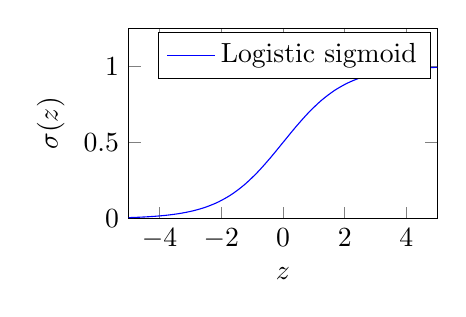
\begin{tikzpicture}
			\begin{axis}[width=5.5cm,height=4cm,ylabel=$\sigma(z)$,xlabel=$z$,ymin=0,ymax=1.25,xmin=-5,xmax=5]
				\addplot[blue,smooth] {1/(1+exp(-x))};
				\addlegendentry{Logistic sigmoid}
			\end{axis}
		\end{tikzpicture}
	}
	\subfigure[Hyperbolic tangent activation function.]{
		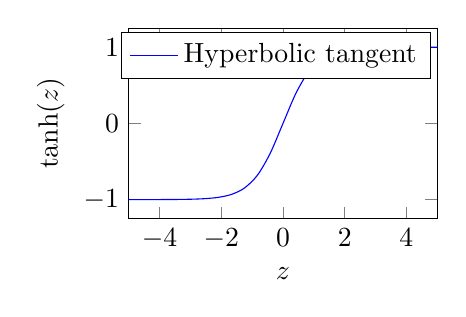
\begin{tikzpicture}
			\begin{axis}[width=5.5cm,height=4cm,ylabel=$\tanh(z)$,xlabel=$z$,ymin=-1.25,ymax=1.25,xmin=-5,xmax=5]
				\addplot[blue,smooth] {tanh(x)};
				\addlegendentry{Hyperbolic tangent}
			\end{axis}
		\end{tikzpicture}
	}
	\subfigure[Logistic sigmoid activation function.]{
    		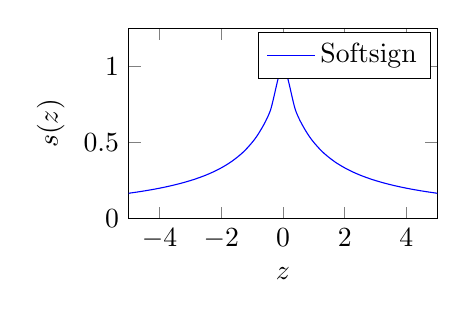
\begin{tikzpicture}
			\begin{axis}[width=5.5cm,height=4cm,ylabel=$s(z)$,xlabel=$z$,ymin=0,ymax=1.25,xmin=-5,xmax=5]
				\addplot[blue,smooth] {1/(1 + abs(x))};
				\addlegendentry{Softsign}
			\end{axis}
		\end{tikzpicture}
	}
	\subfigure[Rectified hyperbolic tangent activation function.]{
		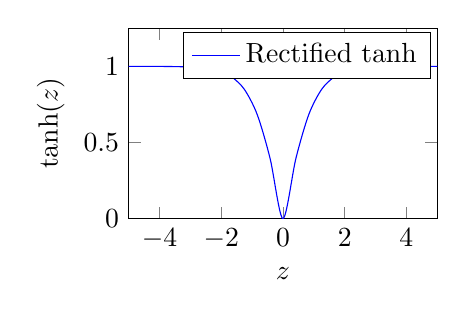
\begin{tikzpicture}
			\begin{axis}[width=5.5cm,height=4cm,ylabel=$\abs{\tanh(z)}$,xlabel=$z$,ymin=0,ymax=1.25,xmin=-5,xmax=5]
				\addplot[blue,smooth] {abs(tanh(x))};
				\addlegendentry{Rectified $\tanh$}
			\end{axis}
		\end{tikzpicture}
	}
    	\caption[Sigmoidal activation functions.]{Common used activation functions include the logistic sigmoid $\sigma(z)$ defined in equation \eqref{eq:logistic-sigmoid} and the hyperbolic tangent $tanh(z)$. More recently used activation functions are the softsign of equation \eqref{eq:softsign} and the rectified hyperbolic tangent.}
    	\label{fig:sigmoid-tanh}
\end{figure}

\subsection{Supervised Training}
\label{subsec:supervised-training}

Supervised training is the problem of determining the network weights to approximate a specific target mapping $g$. In practice, $g$ may be unknown such that the mapping is given by a set of training data. The training set
\begin{align}
	T_S := \{(x_n, t_n) : 1 \leq n \leq N\}
\end{align}
comprises both input values $x_n$ and corresponding desired, possibly noisy, output values $t_n \approx g(x_n)$ \cite{Haykin:2005}.

% In unsuperivsed training, the training set does not contain desired output values and the network has to find similarities and regularities within the training set by itself \cite{Haykin:2005}. We review unsupervised training of convolutional neural networks in section \ref{subsec:unsupervised-training}.

\subsubsection{Error Measures}

Training is accomplished by adjusting the weights $w$ of the neural network to minimize a chosen objective function which can be interpreted as error measure between network output $y(x_n)$ and desired target output $t_n$. Popular choices for classification include the sum-of-squared error measure given by
\begin{align}
	E(w) = \sum_{n = 1}^N E_n(w) = \sum_{n = 1}^N \sum_{k = 1}^C (y_k(x_n,w) - t_{n,k})^2,
\end{align}
and the cross-entropy error measure given by
\begin{align}
	E(w) = \sum_{n = 1}^N E_n(w) = \sum_{n = 1}^N \sum_{k = 1}^C t_{n,k} \log(y_k(x_n,w)),
\end{align}
where $t_{n,k}$ is the $k^{\text{th}}$ entry of the target value $t_n$. Details on the choice of error measure and their properties can be found in \cite{Bishop:1995}.

\subsubsection{Training Protocols}

\cite{DudaHartStork:2001} considers three training protocols:
\begin{description}
	\item[Stochastic training] An input value is chosen at random and the network weights are updated based on the error~$E_n(w)$.
	\item[Batch training] All input values are processed and the weights are updated based on the overall error $E(w) = \sum_{n=1}^N E_n(w)$.
	\item[Online training] Every input value is processed only once and the weights are updated using the error~$E_n(w)$.
\end{description}
Further discussion of these protocols can be found in \cite{Bishop:2006} and \cite{DudaHartStork:2001}. A common practice (e.g. used for experiments in \cite{GlorotBordesBengio:2011}, \cite{GlorotBengio:2010}) combines stochastic training and batch training:
\begin{description}
	\item[Mini-batch training] A random subset $M \subseteq \{1,\ldots,N\}$ (mini-batches) of the training set is processed and the weights are updated based on the cumulative error $E_M(w) := \sum_{n \in M} E_n(w)$.
\end{description}
% In our discussion of network training, we consider stochastic training and, thus, discuss how to minimize the error $E_n$ for a chosen pattern $x_n$. Note, that the following concepts are easily applied both on batch and mini-batch training, as well.

\subsubsection{Parameter Optimization}
\label{subsubsec:parameter-optimization}

Considering stochastic training we seek to minimize $E_n$ with respect to the network weights $w$. % Although $E_n$ is a nonlinear function in the weights and may have multiple local minima, we are interested in a global minimum \cite[p.~253-256]{Bishop:2006}.
The necessary criterion can be written as
\begin{align}
	\frac{\partial E_n}{\partial w} = \nabla E_n(w) \overset{!}{=} 0
\end{align}
where $\nabla E_n$ is the gradient of the error $E_n$.

Due to the complexity of the error $E_n$, a closed-form solution is usually not possible and we use an iterative approach. Let $w[t]$ denote the weight vector in the $t^{\text{th}}$ iteration. In each iteration we compute a weight update $\Delta w[t]$ and update the weights accordingly \cite[p.~236-237]{Bishop:2006}:
\begin{align}
	w[t+1] = w[t] + \Delta w[t].
\end{align}
From unconstrained optimization we have several optimization techniques available. Gradient descent is a first-order method, this means it uses only information of the first derivative of $E_n$ and can, thus, be used in combination with error backpropagation as described in section \ref{subsubsec:error-backproagation}, whereas Newton's method is a second-order method and needs to evaluate the Hessian matrix $H_n$ of $E_n$\footnote{The Hessian matrix $H_n$ of a the error $E_n$ is the matrix of second-order partial derivatives: $\left(H_n\right)_{r,s} = \frac{\partial^2 E_n}{\partial w_r \partial w_s}$} (or an appropriate approximation of the Hessian matrix) in each iteration step.
\begin{description}
	\item[Gradient descent] Gradient descent is motivated by the idea to take a step in the direction of the steepest descent, that is the direction of the negative gradient, to reach a minimum \cite[p.~263-267]{Bishop:1995}. This principle is illustrated by figure \ref{fig:gradient-descent}. Therefore, the weight update is given by
		\begin{align}
			\Delta w[t] = - \gamma \frac{\partial E_n}{\partial w[t]} = - \gamma \nabla E_n (w[t])
		\end{align}
		where $\gamma$ is the learning rate. As discussed in \cite[p.263-272]{Bishop:2006}, this approach has several difficulties, for example how to choose the learning rate to get fast learning but at the same time avoid oscillation\footnote{Oscillation occurs if the learning rate is chosen too large such that the algorithm successively oversteps the minimum.}.
	\item[Newton's method] Although there are some extensions of gradient descent available, second-order methods promise faster convergence because of the use of second-order information \cite{BeckerLeCun:1989}. When using Newton's method, the weight update $\Delta w[t]$ is given by
	\begin{align}
		\Delta w[t] = - \gamma \left(\frac{\partial^2 E_n}{\partial w[t]^2}\right)^{-1} \frac{\partial E_n}{\partial w[t]} = - \gamma \left(H_n(w[t])\right)^{-1} \nabla E_n(w[t])
	\end{align}
	where $H_n(w[t])$ is the Hessian matrix of $E_n$ and $\gamma$ describes the learning rate. The drawback of this method is the evaluation and inversion of the Hessian matrix\footnote{An algorithm to evaluate the Hessian matrix based on error backpropagation as introduced in section \ref{subsubsec:error-backproagation} can be found in \cite{Bishop:1992}. The inversion of an $n \times n$ matrix has complexity $\mathcal{O}(n^3)$ when using the LU decomposition or similar techniques.} which is computationally expensive~\cite{BeckerLeCun:1989}.
\end{description}

\begin{SCfigure}[2\sidecaptionrelwidth][t]
	\centering
	\begin{tikzpicture}[samples=100,smooth]
		\begin{scope}
			\clip(-4,-1) rectangle (4,4);
			\draw plot[domain=0:360] ({cos(\x)*sqrt(20/(sin(2*\x)+2))},{sin(\x)*sqrt(20/(sin(2*\x)+2))});
			\draw plot[domain=0:360] ({cos(\x)*sqrt(16/(sin(2*\x)+2))},{sin(\x)*sqrt(16/(sin(2*\x)+2))});
			\draw plot[domain=0:360] ({cos(\x)*sqrt(12/(sin(2*\x)+2))},{sin(\x)*sqrt(12/(sin(2*\x)+2))});
			\draw plot[domain=0:360] ({cos(\x)*sqrt(8/(sin(2*\x)+2))},{sin(\x)*sqrt(8/(sin(2*\x)+2))});
			\draw plot[domain=0:360] ({cos(\x)*sqrt(4/(sin(2*\x)+2))},{sin(\x)*sqrt(4/(sin(2*\x)+2))});
			\draw plot[domain=0:360] ({cos(\x)*sqrt(1/(sin(2*\x)+2))},{sin(\x)*sqrt(1/(sin(2*\x)+2))});
			\draw plot[domain=0:360] ({cos(\x)*sqrt(0.0625/(sin(2*\x)+2))},{sin(\x)*sqrt(0.0625/(sin(2*\x)+2))});
			
			\draw[-latex new,arrow head=0.25cm,blue,ultra thick] (-2,3.65) to (-1.93,3);
			\draw[-latex new,arrow head=0.25cm,blue,ultra thick] (-1.93,3) to (-1.75,2.4);
			\draw[-latex new,arrow head=0.25cm,blue,ultra thick] (-1.75,2.4) to (-1.5,1.8);
			\draw[-latex new,arrow head=0.25cm,blue,ultra thick] (-1.5,1.8) to (-1.15,1.3);
			
			\node at (-1.4,3.8){$w[0]$};
			\node at (-1.2,3.2){$w[1]$};
			\node at (-1.05,2.6){$w[2]$};
			\node at (-0.8,2){$w[3]$};
			\node at (-0.6,1.4){$w[4]$};
		\end{scope}
	\end{tikzpicture}
	\caption[The principle of gradient descent.]{Illustrated using a quadratic function to minimize, the idea of gradient descent is to follow the negative gradient at the current position as it describes the direction of the steepest descent. The learning rate $\gamma$ describes the step size taken in each iteration step. Therefore, gradient descent describes a first-order optimization technique.}
	\label{fig:gradient-descent}
\end{SCfigure}

\subsubsection{Weight Initialization}
\label{sububsec:weight-initialization}

As we use an iterative optimization technique, the initialization of the weights $w$ is crucial. \cite[p.~311-312]{DudaHartStork:2001} suggest choosing the weights randomly in the range
\begin{align}
	\label{eq:weight-initialization}
	- \frac{1}{\sqrt{m^{(l-1)}}} < w_{i,j}^{(l)} < \frac{1}{\sqrt{m^{(l-1)}}}.
\end{align}
This result is based on the assumption that the inputs of each unit are distributed according to a Gaussian distribution and ensures that the actual input is approximately of unity order. Given logistic sigmoid activation functions, this is meant to result in optimal learning \cite[p.~311-312]{DudaHartStork:2001}.
% \footnote{In general, the Gaussian distribution of a $n$ dimensional random variable $x$ is given by \begin{align}G(x|\mu,\Sigma) = \frac{1}{\sqrt{(2\pi)^n |\Sigma|}} \exp\left\{ -\frac{1}{2}(x-\mu)\Sigma^{-1}(x-\mu)^T\right\}\end{align} where $|\Sigma|$ denotes the determinant of $\Sigma$.}
% This result is based on the following considerations assuming the logistic sigmoid activation function. We want to initialize the weights such that we achieve fast and uniform learning, where uniform learning means that the weights should reach their final state at approximately the same time. Thus, the actual input of a unit should not be too large causing the logistic sigmoid to saturate resulting in $\sigma'(z)$ being very small. In addition, the actual input should not bee too small such that the logistic sigmoid is nearly linear. Both cases result in slow learning. When choosing the weights as suggested in equation \eqref{eq:weight-initialization} and assuming the inputs of a unit to be distributed according to a Gaussian\footnote{In general, the Gaussian distribution of a $n$ dimensional random variable $x$ is given by \begin{align}G(x|\mu,\sum) = \frac{1}{\sqrt{(2\pi)^n |\sum|}} \exp\left\{ -\frac{1}{2}(x-\mu)\sum^{-1}(x-\mu)^T\right\}\end{align} where $|\sum|$ denotes the determinant of $\sum$. In the one dimensional case this constitutes to $G(x|\mu,\sigma) = \frac{1}{\sqrt{2\pi}\sigma} \exp\left\{\frac{(x - \mu)}{2\sigma^2}\right\}$ where $\mu$ is the mean of the random variable $x$, and $\sigma^2$ the corresponding variance.} with zero mean and unity variance, the actual input will be approximately of unity order, resulting in optimal learning \cite[p.~311-312]{DudaHartStork:2001}.

In \cite{GlorotBengio:2010} an alternative initialization scheme called normalized initialization is introduced. We choose the weights randomly in the range
\begin{align}
	\label{eq:normalized-initialization}
	- \frac{\sqrt{6}}{\sqrt{m^{(l-1)} + m^{(l)}}} < w_{i,j}^{(l)} < \frac{\sqrt{6}}{\sqrt{m^{(l-1)} + m^{(l)}}}.
\end{align}
The derivation of this initialization scheme can be found in \cite{GlorotBengio:2010}. Experimental results in \cite{GlorotBengio:2010} demonstrate improved learning when using normalized initialization.

An alternative to these weight initialization schemes is given by layer-wise unsupervised pre-training as discussed in \cite{ErhanBengioCourvilleManzagolVincentBengio:2010}. We discuss unsupervised training in section \ref{subsec:unsupervised-training}.

\subsubsection{Error Backpropagation}
\label{subsubsec:error-backproagation}

Algorithm \ref{alg:error-backpropagation}, proposed in \cite{RumelhartHintonWilliams:1986}, is used to evaluate the gradient $\nabla E_n (w[t])$ of the error function $E_n$ in each iteration step. More details as well as a thorough derivation of the algorithm can be found in \cite{Bishop:1995} or \cite{RumelhartHintonWilliams:1986}. 

\begin{algorithm}[Error Backpropagation]
	\label{alg:error-backpropagation}
	\begin{enumerate}[1.]
		\item Propagate the input value $x_n$ through the network to get the actual input and output of each unit.
		\item Calculate the so called errors $\delta_i^{(L+1)}$ \cite[p.~241-245]{Bishop:2006} for the output units:
		\begin{align}
			\delta_i^{(L+1)} := \frac{\partial E_n}{\partial y_i^{(L+1)}} f'(z_i^{(L+1)}).
		\end{align}
		\item Determine $\delta _i ^{(l)}$ for all hidden layers $l$ by using error backpropagation:
		\begin{align}
			\delta _i ^{(l)} := f' (z_i^{(l)}) \sum _{k = 1} ^{m^{(l+1)}} w_{i,k}^{(l+1)} \delta _k ^{(l+1)}.
		\end{align}
		\item Calculate the required derivatives:
		\begin{align}
			\label{eq:backprop-derivative}
			\frac{\partial E_n}{\partial w_{j,i}^{(l)}} = \delta _j ^{(l)} y_i^{(l-1)}.
		\end{align}
	\end{enumerate}
\end{algorithm}

\subsection{Unsupervised Training}
\label{subsec:unsupervised-training}

In unsupervised training, given a training set
\begin{align}
	T_U := \{x_n : 1 \leq n \leq N\}
\end{align}
without desired target values, the network has to find similarities and regularities within the data by itself.

% For deep neural networks, unsupervised training has several applications when labeled training data is given, as well. Weight initialization by unsupervised pre-training, followed by supervised fine-tuning can be interpreted as regularization method as discussed in section \ref{subsubsec:unsupervised-pretraining}.

Among others, unsupervised training of deep architectures can be accomplished based on Restricted Boltzman Machines\footnote{A brief introduction to Restricted Boltzman Machines can be found in \cite{Bengio:2009}.} or auto-encodes \cite{Bengio:2009}. We focus on auto-encoders.

\subsubsection{Auto-Encoders}
\label{subsubsec:auto-encoders}

Auto-encoders, also called auto-associators \cite{Bengio:2009}, are two-layer perceptrons with the goal to compute a representation of the input in the first layer from which the input can accurately be reconstructed in the output layer. Therefore, no desired target values are needed -- auto-encoders are self-supervised \cite{Bengio:2009}.
\begin{SCfigure}[\sidecaptionrelwidth][t!]
	\centering
	\begin{tikzpicture}[shorten >=1pt]
		\tikzstyle{unit}=[draw,shape=circle,minimum size=1.15cm]
		\tikzstyle{hidden}=[draw,shape=circle,minimum size=1.15cm]

		\node[unit](x0) at (0,3.5){$x_0$};
		\node[unit](x1) at (0,2){$x_1$};
		\node(dots) at (0,1){\vdots};
		\node[unit](xd) at (0,0){$x_D$};

		\node[hidden](h0) at (3,4){$c_0(x)$};
		\node[hidden](h1) at (3,2.5){$c_1(x)$};
		\node(dots) at (3,1.5){\vdots};
		\node[hidden](hm) at (3,-0.5){$c_m(x)$};

		\node[unit](y1) at (6,3.5){$\hat{x}_1$};
		\node[unit](y2) at (6,2){$\hat{x}_2$};
		\node(dots) at (6,1){\vdots};	
		\node[unit](yc) at (6,0){$\hat{x}_C$};

		\draw[-latex new,arrow head=0.15cm] (x0) -- (h1);
		\draw[-latex new,arrow head=0.15cm] (x0) -- (hm);

		\draw[-latex new,arrow head=0.15cm] (x1) -- (h1);
		\draw[-latex new,arrow head=0.15cm] (x1) -- (hm);

		\draw[-latex new,arrow head=0.15cm] (xd) -- (h1);
		\draw[-latex new,arrow head=0.15cm] (xd) -- (hm);

		\draw[-latex new,arrow head=0.15cm] (h0) -- (y1);
		\draw[-latex new,arrow head=0.15cm] (h0) -- (yc);
		\draw[-latex new,arrow head=0.15cm] (h0) -- (y2);

		\draw[-latex new,arrow head=0.15cm] (h1) -- (y1);
		\draw[-latex new,arrow head=0.15cm] (h1) -- (yc);
		\draw[-latex new,arrow head=0.15cm] (h1) -- (y2);

		\draw[-latex new,arrow head=0.15cm] (hm) -- (y1);
		\draw[-latex new,arrow head=0.15cm] (hm) -- (yc);

		\draw [decorate,decoration={brace,amplitude=10pt},xshift=-4pt,yshift=0pt] (-0.5,4) -- (0.75,4) node [black,midway,yshift=+0.6cm]{input layer};
		\draw [decorate,decoration={brace,amplitude=10pt},xshift=-4pt,yshift=0pt] (2.5,4.5) -- (3.75,4.5) node [black,midway,yshift=+0.6cm]{representation layer};
		\draw [decorate,decoration={brace,amplitude=10pt},xshift=-4pt,yshift=0pt] (5.5,4) -- (6.75,4) node [black,midway,yshift=+0.6cm]{reconstruction layer};
	\end{tikzpicture}
	\caption[Network graph of an auto-encoder.]{An auto-encoder is mainly a tow-layer perceptron with $m := m^{(1)}$ hidden units and the goal to compute a representation $c(x)$ in the first layer from which the input can accurately be reconstructed in the output layer.}
	\label{fig:twolayer-perceptron}
\end{SCfigure}
In the hidden layer, consisting of $m := m^{(1)}$ units, an auto-encoder computes a representation $c(x)$ from the input $x$ \cite{Bengio:2009}:
\begin{align}
	c_i(x) = \sum_{k = 0} ^D w_{i,k}^{(1)} x_k.
\end{align}
The output layer tries to reconstruct the input from the representation given by $c(x)$:
\begin{align}
	\hat{x}_i = d_i(c(x)) = \sum_{k = 0} ^m w_{i,k}^{(2)} c_k(x).
\end{align}

As the output of an auto-encoder should resemble its input, it can be trained as discussed in section \ref{subsec:supervised-training} by replacing the desired target values $t_n$ used in the error measure by the input $x_n$. In the case where $m < D$, the auto-encoder is expected to compute a useful, dimensionality-reducing representation of the input. If $m \geq D$, the auto-encoder could just learn the identity such that $\hat{x}$ would be a perfect reconstruction of $x$. However, as discussed in \cite{Bengio:2009}, in practice this is not a problem.

\subsubsection{Layer-Wise Training}
\label{subsubsec:layer-wise-training}

As discussed in \cite{LarochelleBengioLouradourLamblinBottou:2009}, the layers of a neural network can be trained in an unsupervised fashion using the following scheme:
\begin{enumerate}[1.]
	\item For each layer $l = 1, \ldots, L+1$:
	\begin{enumerate}[--]
		\item Train layer $l$ using the approach discussed above taking the output of layer $(l-1)$ as input, associating the output of layer $l$ with the representation $c(y^{(l-1)})$ and adding an additional layer to compute $\hat{y}^{(l)}$.
	\end{enumerate}
\end{enumerate}
% Layer-wise unsupervised training can also be used to initialize the weights for supervised training or as regularization method (see section \ref{subsubsec:unsupervised-pretraining}).

\subsection{Regularization}

% Usually the training set $T$ is split up into the actual training set and the validation set \cite{DudaHartStork:2001}. The neural network is trained using the new training set and its performance is evaluated on the validation set.

It has been shown, that multilayer perceptrons with at least one hidden layer can approximate any target mapping up to arbitrary accuracy \cite{HornikStinchcombeWhite:1989}. Thus, the training data may be overfitted, that is the training error may be very low on the training set but high on unseen data \cite{Bengio:2009}. Regularization describes the task to avoid overfitting to give better generalization performance, meaning that the trained network should also perform well on unseen data  \cite{Haykin:2005}. Therefore, the training set is usually split up into an actual training set and a validation set. The neural network is then trained using the new training set and its generalization performance is evaluated on the validation set \cite{DudaHartStork:2001}.

There are different methods to perform regularization. Often, the training set is augmented to introduce certain invariances the network is expected to learn \cite{KrizhevskySutskeverHinton:2012}. Other methods add a regularization term to the error measure aiming to control the complexity and form of the solution \cite{Bishop:1995}:
\begin{align}
	\hat{E}_n (w) = E_n (w) + \eta P(w)
\end{align}
where $P(w)$ influences the form of the solution and $\eta$ is a balancing parameter.

\subsubsection{$L_p$-Regularization}
\label{subsubsec:lp-regularization}

A popular example of $L_p$-regularization is the $L_2$-regularization\footnote{The $L_2$-regularization is often referred to as weight decay, see \cite{Bishop:1995} for details.}:
\begin{align}
	P(w) = \|w\|_2^2 = w^Tw.
\end{align}
The idea is to penalize large weights as they tend to result in overfitting \cite{Bishop:1995}. In general, arbitrary $p$ can be used to perform $L_p$-regularization. Another example sets $p = 1$\footnote{For $p = 1$, the norm $\|\cdot\|_1$ is defined by $\|w\|_1 = \sum_{k = 1} ^W |w_k|$ where $W$ is the dimension of the weight vector $w$.} to enforce sparsity of the weights, that is many of the weights should vanish:
\begin{align}
	P(w) = \|w\|_1.
\end{align}

\subsubsection{Early Stopping}

While the error on the training set tends to decrease with the number of iterations, the error on the validation set usually starts to rise again once the network starts to overfit the training set. To avoid overfitting, training can be stopped as soon as the error on the validation set reaches a minimum, that is before the error on the validation set rises again \cite{Bishop:1995}. This method is called early stopping.

\subsubsection{Dropout}

In \cite{HintonSrivastavaKrizhevskySutskeverSalakhutdinov:2012} another regularization technique, based on observation of the human brain, is proposed. Whenever the neural network is given a training sample, each hidden unit is skipped with probability $\frac{1}{2}$. This method can be interpreted in different ways \cite{HintonSrivastavaKrizhevskySutskeverSalakhutdinov:2012}. First, units cannot rely on the presence of other units. Second, this method leads to the training of multiple different networks simultaneously. Thus, dropout can be interpreted as model averaging\footnote{Model averaging tries to reduce the error by averaging the prediction of different models \cite{HintonSrivastavaKrizhevskySutskeverSalakhutdinov:2012}.}.

\subsubsection{Weight Sharing}
\label{subsubsec:weight-sharing}

The idea of weight sharing was introduced in \cite{RumelhartHintonWilliams:1986} in the context of the T-C problem\footnote{The T-C problem describes the task of classifying images into those containing a ``T'' and those containing a ``C'' independent of position and rotation \cite{RumelhartHintonWilliams:1986}.}. Weight sharing describes the idea of different units within the same layer to use identical weights. This can be interpreted as a regularization method as the complexity of the network is reduced and prior knowledge may be incorporated into the network architecture. The equality constraint is replaced when using soft weight sharing, introduced in \cite{NowlanHinton:1992}. Here, a set of weights is encouraged not to have the same weight value but similar weight values. Details can be found in \cite{NowlanHinton:1992} and \cite{Bishop:1995}.

When using weight sharing, error backpropagation can be applied as usual, however, equation \eqref{eq:backprop-derivative} changes to
\begin{align}
	\frac{\partial E_n}{\partial w_{j,i}^{(l)}} = \sum _{k = 1} ^{m^{(l)}} \delta_k^{(l)} y_i^{(l-1)}
\end{align}
when assuming that all units in layer $l$ share the same set of weights, that is $w_{j,i}^{(l)} = w_{k,i}^{(l)}$ for $1 \leq j,k \leq m^{(l)}$. Nevertheless, equation \eqref{eq:backprop-derivative} still needs to be applied in the case that the errors need to be propagated to preceding layers \cite{Bishop:2006}.

\subsubsection{Unsupervised Pre-Training}
\label{subsubsec:unsupervised-pretraining}

Results in \cite{ErhanBengioCourvilleManzagolVincentBengio:2010} suggest that layer-wise unsupervised pre-training of deep neural networks can be interpreted as regularization technique\footnote{Another interpretation of unsupervised pre-training is that it initializes the weights in the basin of a good local minimum and can therefore be interpreted as optimization aid \cite{Bengio:2009}.}. Layer-wise unsupervised pre training can be accomplished using a similar scheme as discussed in section~\ref{subsubsec:layer-wise-training}:
\begin{enumerate}[1.]
	\item For each $l = 1, \ldots, L+1$:
	\begin{enumerate}[--]
		\item Train layer $l$ using the approach discussed in section \ref{subsubsec:auto-encoders}.
	\end{enumerate}
	\item Fine-tune the weights using supervised training as discussed in section \ref{subsec:supervised-training}.
\end{enumerate}


A formulation of the effect of unsupervised pre-training as regularization method is proposed in \cite{ErhanManzagolBengioVincent:2009}: The regularization term punishes weights outside a specific region in weight space with an infinite penalty such that
\begin{align}
	P(w) = - \log(p(w))
\end{align}
where $p(w)$ is the prior for the weights, which is zero for weights outside this specific region \cite{ErhanBengioCourvilleManzagolVincentBengio:2010}.

